\chapter{基于CUDA的形态学图像处理}
\section{实验目的与要求}
\begin{enumerate}
    \item 深入理解GPGPU的架构并掌握CUDA编程模型
    \item 使用CUDA实现形态图像处理操作的并行算法
    \item 对程序执行结果进行简单的分析和总结
    \item 根据执行结果和硬件环境提出优化解决方案
    \item 将其与Lab2,Lab3和Lab4的结果进行比较
\end{enumerate}

\section{算法描述}
\par 与上述并行算法不同的是,CUDA使用的是异构的并行算法,由于GPU本身就比较适合进行图像处理,因此预计相对于串行算法的加速比会比较高。同样,按照pthread实验中的方法对于图片进行分块,然后将每一个图片块分配给不同的CUDA block,将块中的不同像素分配给不同的CUDA Thread进行处理。如图\ref{fig:cudaScheme}所示,线程的处理过程与算法ErodeAndDilate相同。
\begin{figure}[htpb]
    \centering
    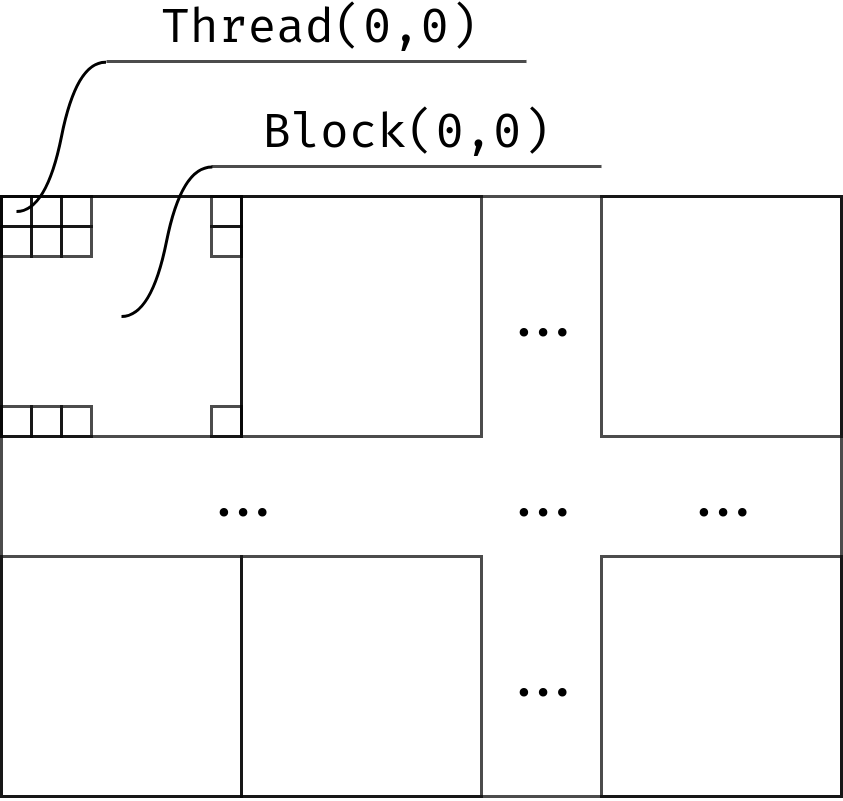
\includegraphics[width=0.4\linewidth]{cudaScheme.png}
    \caption{CUDA块与线程分配}
    \label{fig:cudaScheme}
\end{figure}

\section{实验方案}
\par 编写CUDA程序并进行测试,在编译时需要使用CUDA的包装编译器nvcc进行编译,,在运行时需要保证Nvidia驱动已被正确加载。

\section{实验结果与分析}
\par 图像处理的结果与串行图像处理的结果相同,性能方面,程序在使用分块大小为128,每个像素使用一个线程处理的情况下,处理时间如图\ref{fig:cudaOutput}所示,可以看出,程序只使用了989ms就完成了1000次处理,相对与并行程序加速比达到了44.7,由此可见CUDA是较为适合并行处理图片的。

\begin{figure}[htpb]
    \centering
    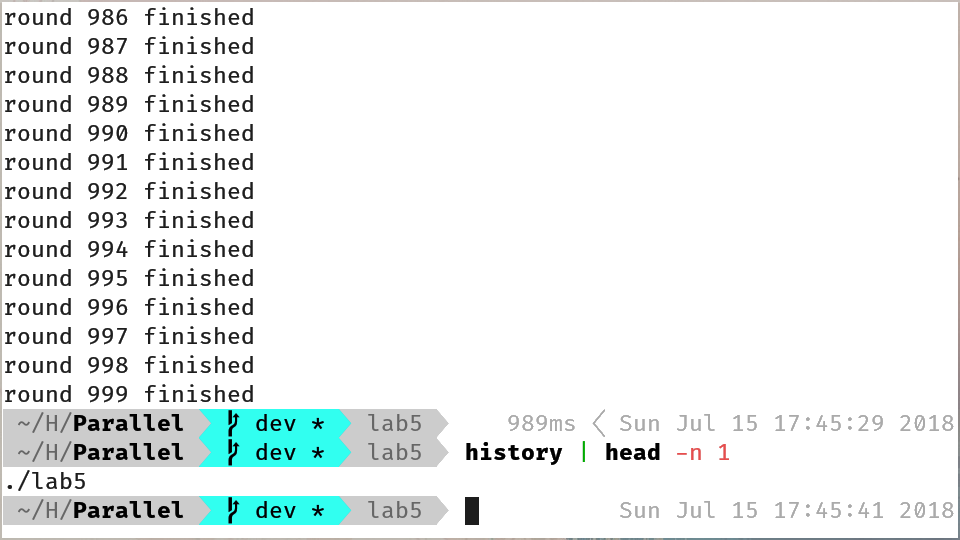
\includegraphics[width=0.9\linewidth]{cudaOutput.png}
    \caption{CUDA程序运行结果}
    \label{fig:cudaOutput}
\end{figure}
\par 由于CUDA架构与仅使用CPU并行的架构完全因此不同,因此不具备与CPU程序在性能上的可比性。在不同的块大小情况下,CUDA程序的最优时间为686ms,相对于串行程序的加速比达到了64.31,由此可见,对于数据易于分块,数据间无依赖的简单数据使用GPU进行处理占有绝对优势。
